\section{Installazione e avvio}
\subsection{Requisiti Server}
\subsubsection{Base}
\noindent Per utilizzare il server è necessario:
\begin{itemize}[label=-]
  \item Installare \href{https://dev.mysql.com/downloads/installer/}{MySQL} sul proprio computer
  \item Eseguire lo script sql presente in \path{KmeansServer/out/artifacts/KmeansServer_jar} se si vuole utilizzare il database di default
  \item Installare \href{https://www.oracle.com/technetwork/java/javase/downloads/jre8-downloads-2133155.html}{JRE} 8
  \item Installare \href{https://www.oracle.com/java/technologies/javase/jdk19-archive-downloads.html}{JDK 19.0.2}
\end{itemize}

\subsubsection{Estensione}
\noindent Nel caso di host proprietario del server i requisiti sono gli stessi del server della versione base, per utilizzare il database di default il percorso è \path{KmeansServer/out/artifacts/Server_main_jar}. Nel caso di fruizione del server mediante indirizzo fornito dal team di sviluppo non sarà necessaria alcuna azione.

\subsection{Requisiti Client}
\subsubsection{CLI}
\noindent Per utilizzare il client è necessario:
\begin{itemize}[label=-]
  \item Installare \href{https://www.oracle.com/technetwork/java/javase/downloads/jre8-downloads-2133155.html}{JRE} 8  
  \item Server in ascolto
\end{itemize}

\subsubsection{App}
\noindent Per utilizzare il client app è necessario:
\begin{itemize}[label=-]
  \item Un dispositivo Android con sistema operativo Android 5.0 Lollipop o superiore
  \item Installare l'applicazione: trasferire l'APK presente nel percorso \path{KmeansClient/app/build/outputs/apk/debug/KmeansClient.apk} sullo smartphone. Aprire il file APK e installare l'applicazione. Se necessario abilitare l'installazione di applicazioni da sorgenti sconosciute e dare l'ok nel caso in cui l'installazione venga bloccata da Play Protect.
  \item Server in ascolto
\end{itemize}


\subsection{Avvio server}
\subsubsection{CLI}
\noindent Per avviare il server e' necessario eseguire il file \textit{server.bat} presente nel percorso \path{KmeansServer/out/artifacts/KmeansServer_jar}. In alternativa è possibile avviarlo da riga di comando tramite il comando \textit{java -jar server.jar} eseguito nella cartella dove si trova il \textit{jar}.

\subsubsection{App}
\noindent Per avviare il server e' necessario eseguire il file \textit{server.bat} presente nel percorso \path{KmeansServer/out/artifacts/Server_main_jar}. In alternativa è possibile avviarlo da riga di comando tramite il comando \textit{java -jar server.jar} eseguito nella cartella dove si trova il \textit{jar}.

\subsection{Avvio client}
\subsubsection{CLI}
\noindent Per avviare il client da riga di comando è necessario eseguire il file \textit{client.bat} presente nel percorso \path{KmeansClient/out/artifacts/KmeansClient_jar}. Questa modalità di avvio connetterà il client ad un server in esecuzione sulla propria macchina sulla porta 8080. Per specificare un altro server a cui connettersi è necessario
avviare il client da riga di comando tramite il comando \textit{java -jar client.jar indirizzo\_ip porta} o inserendo tale comando nel file \textit{bat}.


\subsubsection{App}
\noindent Per avviare il client app basta avviare l'applicazione sul proprio smartphone ed inserire indirizzo ip e porta del server a cui ci si vuole connettere:
\begin{figure}[H]
  \centering
  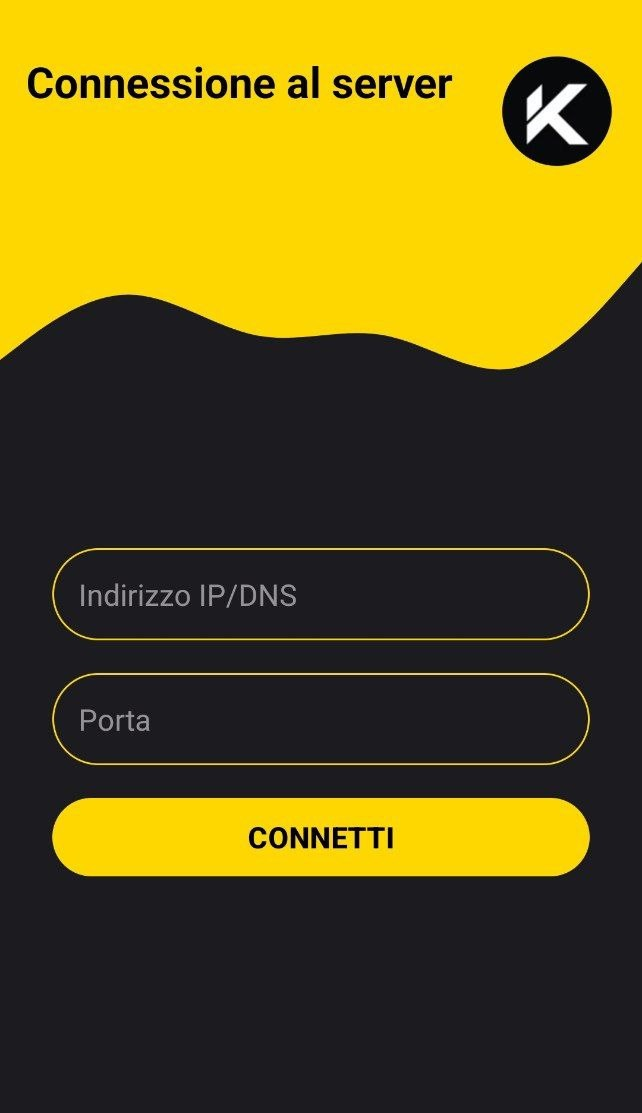
\includegraphics[scale=0.25]{img/app1.png}
\end{figure}
